%%%%%%%%%%%%%%%%%%%%%%%%%%%%%%%%%%%%%%%%%%%%%%%%%%%%%%%%%%%%%%%%%%%%%%%%%%%%%%%%
%2345678901234567890123456789012345678901234567890123456789012345678901234567890
%        1         2         3         4         5         6         7         8

\documentclass[letterpaper, 10 pt, conference]{ieeeconf}  % Comment this line out if you need a4paper

%\documentclass[a4paper, 10pt, conference]{ieeeconf}      % Use this line for a4 paper

\IEEEoverridecommandlockouts                              % This command is only needed if
                                                          % you want to use the \thanks command

\overrideIEEEmargins                                      % Needed to meet printer requirements.

%In case you encounter the following error:
%Error 1010 The PDF file may be corrupt (unable to open PDF file) OR
%Error 1000 An error occurred while parsing a contents stream. Unable to analyze the PDF file.
%This is a known problem with pdfLaTeX conversion filter. The file cannot be opened with acrobat reader
%Please use one of the alternatives below to circumvent this error by uncommenting one or the other
%\pdfobjcompresslevel=0
%\pdfminorversion=4

% See the \addtolength command later in the file to balance the column lengths
% on the last page of the document

% The following packages can be found on http:\\www.ctan.org
\usepackage{graphics} % for pdf, bitmapped graphics files
\usepackage{epsfig} % for postscript graphics files
%\usepackage{mathptmx} % assumes new font selection scheme installed
%\usepackage{times} % assumes new font selection scheme installed
%\usepackage{amsmath} % assumes amsmath package installed
%\usepackage{amssymb}  % assumes amsmath package installed

\usepackage{amsmath}
\usepackage{amsfonts}%
\usepackage{amssymb}%
\usepackage{color}
\usepackage{graphicx}
\usepackage{subeqnarray}
\usepackage{arydshln}
\usepackage{chemarrow}

\newtheorem{theorem}{Theorem}
\newtheorem{lemma}{Lemma}
\newtheorem{definition}{Definition}
\newtheorem{cor}{Corollary}
\newtheorem{example}{Example}
\newtheorem{opt}{Optimization Problem}
\newtheorem{proposition}{Proposition}
\newtheorem{remark}{Remark}


\title{\LARGE \bf
A Feedback SIRD Model  for the Spread of Infectious Disease with Application to COVID-19 Pandemic
}

\author{Daniel March, Jeston Bond and Gentian Buzi% <-this % stops a space
\thanks{Daniel March, Jeston Bond and Gentian Buzi are with the Department of Mathematics and Computer Science,
       Biola University, 13800 Biola Ave, La Mirada, CA 90639, USA
        {\tt\small daniel.march, jeston.bond, genti.buzi@biola.edu}}%
}


\begin{document}



\maketitle
\thispagestyle{empty}
\pagestyle{empty}


%%%%%%%%%%%%%%%%%%%%%%%%%%%%%%%%%%%%%%%%%%%%%%%%%%%%%%%%%%%%%%%%%%%%%%%%%%%%%%%%
\begin{abstract}

The COVID-19 global pandemic has highlighted the importance of identifying effective ways to control the spread of an infectious disease in a population. A solid understanding of the dynamics and the underlying mechanisms that govern this spread is an important step toward such a goal. Susceptible-Infected-Recovered (SIR) models and their variants have played an important role in providing such insight. However, these models have limited explanatory and predictive power due to policy and behavior changes over time. Here we present a modified version of the standard SIR models by introducing feedback in the disease transmission rate. We apply this model to publicly available COVID-19 US and international infection data. We show this model is more robust to parameter variations due to public health interventions and has much better explanatory and predictive power


\end{abstract}


%%%%%%%%%%%%%%%%%%%%%%%%%%%%%%%%%%%%%%%%%%%%%%%%%%%%%%%%%%%%%%%%%%%%%%%%%%%%%%%%
\section{INTRODUCTION}


\section{A feedback model for the early spread of infectious disease}

\subsection{Modeling}

 

\subsection{Feedback Model}



\section{Fitting the model to COVID-19 infection data}



\subsection{COVID-19 Infection Data and Non-Pharmaceutical Interventions (NPIs)}

The data to evaluate our model is from OWID (Our World in Data), a publically available database, from which we extract data about COVID-19 for different countries (i.e. total infections, daily tests, population). In order to fit our model to the data we must interpolate the current infections of a given region. We can model the current infections as

\begin{equation*}
I(t) = I_{total}(t) - R_{total}(t) - D_{total}(t)
\end{equation*}

Which is to say the current infected is any of the total infected who have not yet recovered or died. Total deaths and total tested positive individuals are reported but we must estimate the recovered population. To do this we assume $R_{total}$ is a shifted version of $I_{total}$. To determine the shift we consider that for most infections are resolved within 10 days of becoming symptomatic and for 3 days prior to syptoms the individual is infectious. Therefore, we use a shift of 13 to dertermine the recovered individuals which returns us with a realistic infection curve.

\begin{equation*}
R_{total}(t + s) = I_{total}(t) - D_{total}(t+s)
\end{equation*}

Next, we must consider that the given infection data for a region is highly dependent on the number of tests. Since relatively low testing was performed during the beginning of the pandemic, we expect the reported infections during this time to be an underestimation of the true numbers. There are multiple methods to estimate the true number of infections. We advocate for using the number of tests to scale each day accordingly. This is done by 

\begin{equation*}
I_{estimated}(t) = \alpha I_{reported}(t) / Tests(t)
\end{equation*}

A similar approach using test data has previously been applied successfully \cite{Ironse2103272118}. The scaling, $\alpha$ of $I_{estimated}$ is arbitrary and does not affect our model or it's predictive power. To normalize the data we let the scaler be such that the total infections over the period = .25. The results yielded by this method are similar in effect to other methods such as REMEDID \cite{GarcaGarca2021RetrospectiveMT}, which uses death data and are compared in Figure 1.


%%%% FigureX%%%
\begin{figure}
\begin{centering}
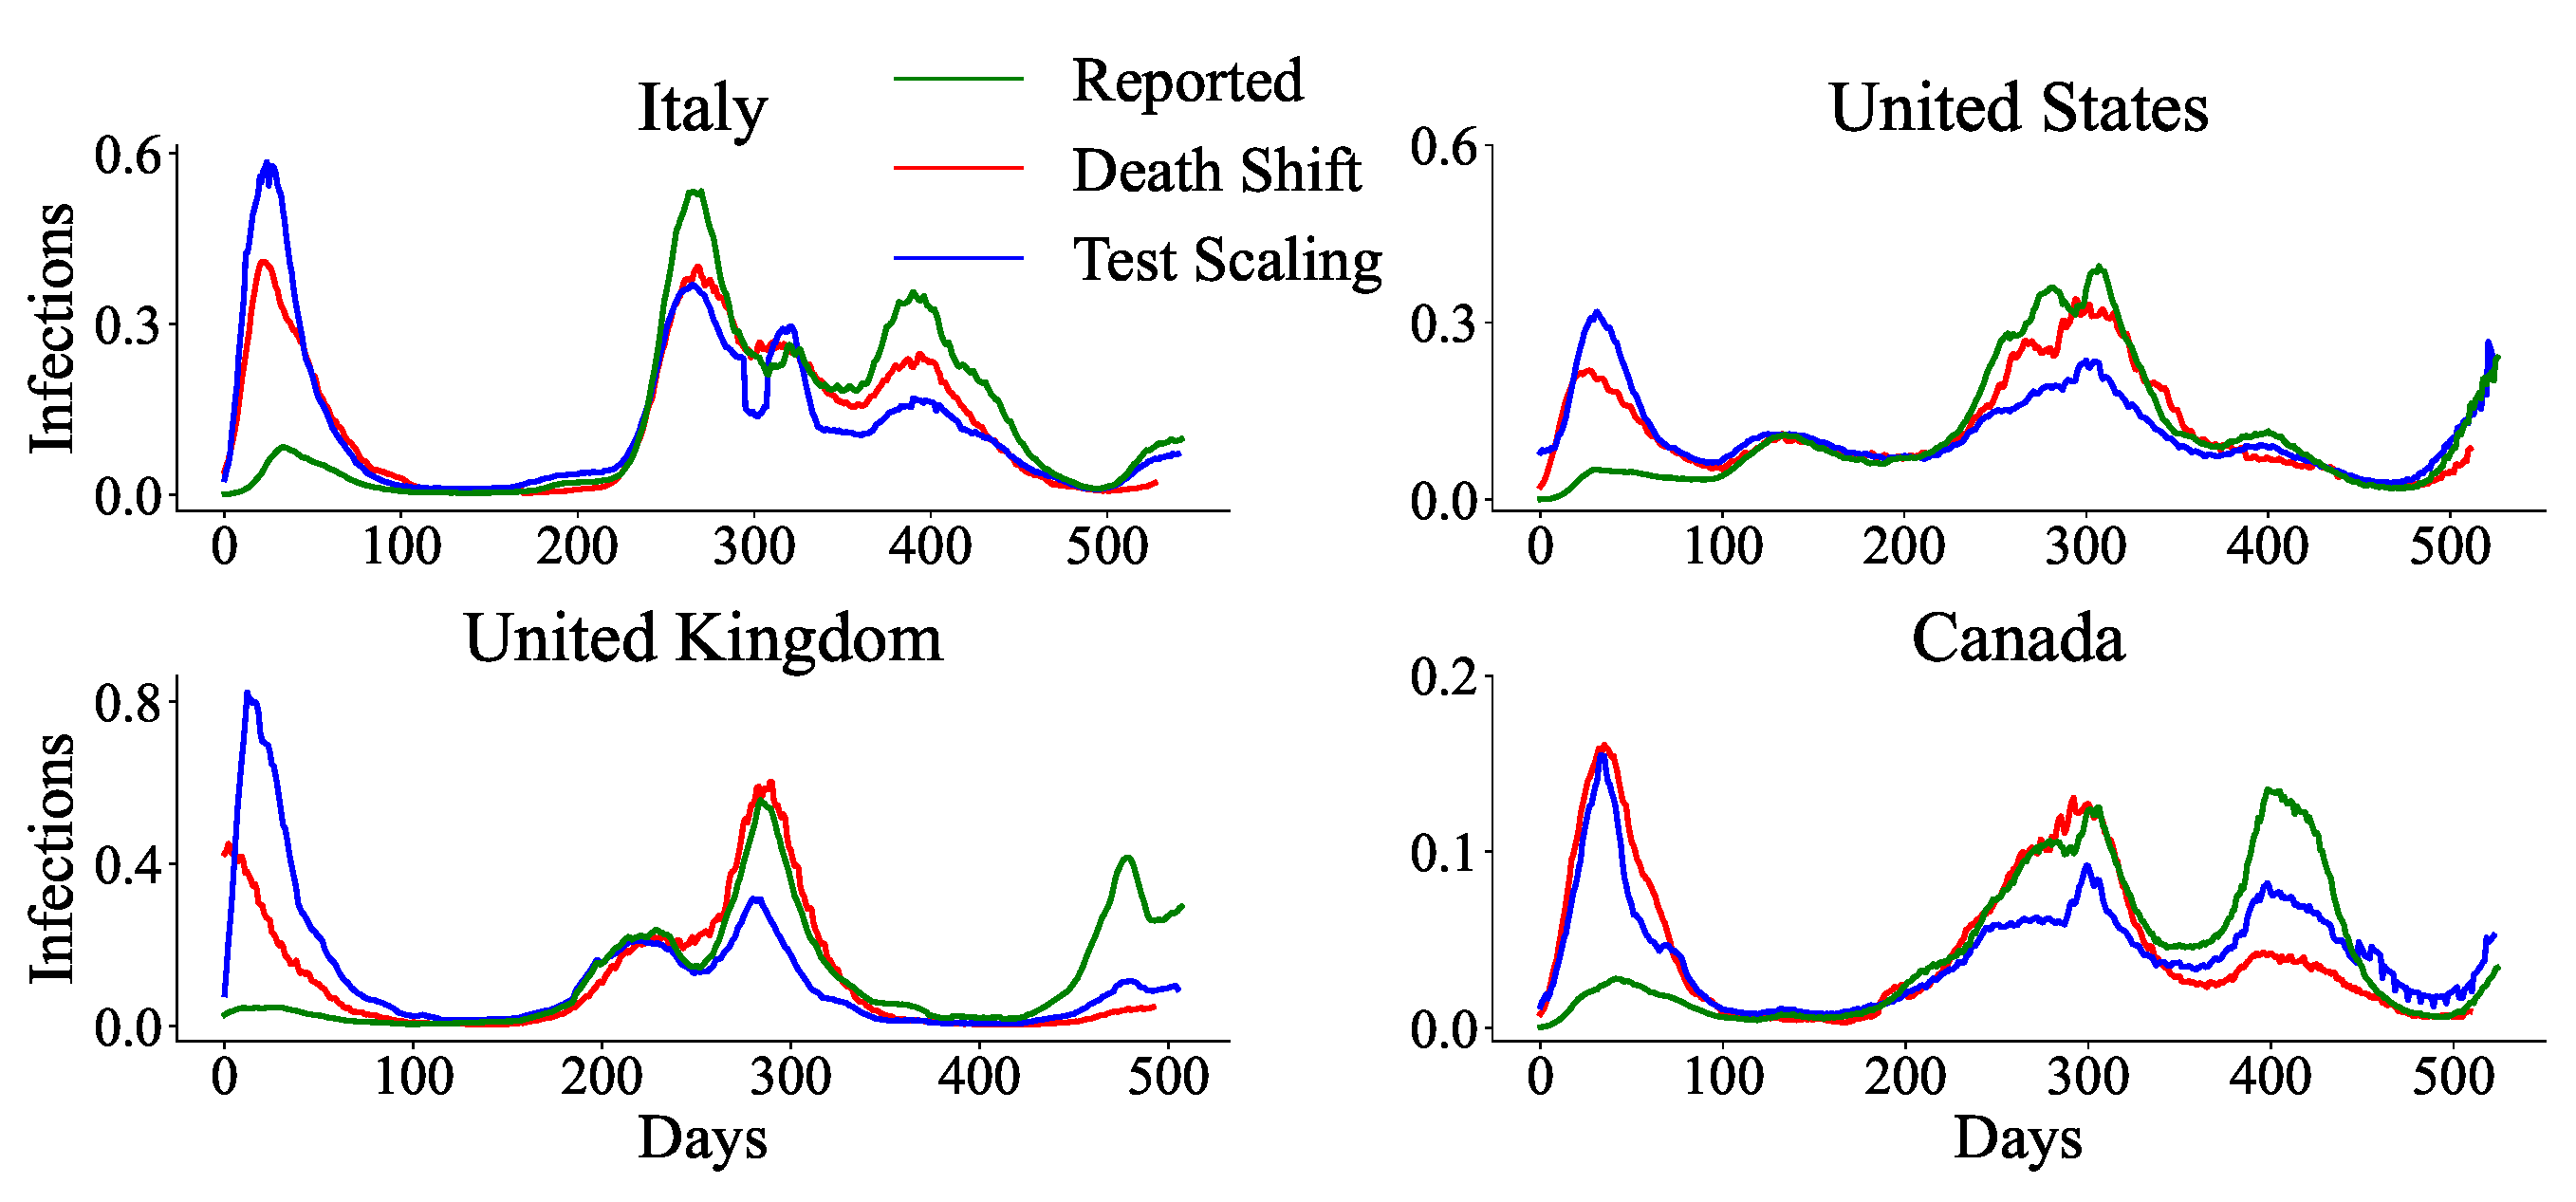
\includegraphics[width=3.6in]{DifferentMethods}
\par\end{centering}
\caption{\label{fig:InfectionMethods} Comparing  methods of estimating current infections. Our method (blue) corrects the reported number based on the number of tests performed. This compensates for the under reporting of infections during the beginning of the pandemic. Another method using death scaling (red), yields different but comparable results. For all methods, scaling is arbitrary and purely serve as comparisons.}
\end{figure}
%%%% FigureXend%%%


\subsection{Data Fitting Procedure}

In order to fit the data, we must find the optimal parameters and simulate our model. Our parameters we need to fit are $A(0)$, $I(0)$, $\kappa_1$, $\kappa_2$, $\kappa_3$, $\beta_1$, $\beta_2$, and $\beta_3$. To do this we begin with reasonable random starting values of parameters and optimize using the Nelder-Mead method from scipy.optimize. This method is used since it is effective at escaping local minima, which our model is prone to having. This is done several times to explore a wide range of the space and to ensure a good fit. We are optimizing for a least squared error function.

Simulate using:
\begin{equation*} 
\begin{split}
&\dot{A}(t) = {\frac{\beta_1}{1+(\beta_2 I)^{\beta_3}}}A(t) - \kappa_1 A(t) \\
& \dot{I}(t) = \kappa_2 A(t) - \kappa_2 I(t)
\end{split}
\end{equation*}

Minimize:
\begin{equation*}
\frac{1}{T} \sum_{t=0}^{T}(I_{actual}(t) - I(t))^2
\end{equation*}

\section{Analysis}

\subsection{Performance of the Model}

Running our model on data from various countries yields promising results and can be seen in FIGURE TO BE ADDED. Typically the position and height of the major waves is captured well. This implies there is feedback on the number of infections, meaning the populus reacts to the recent infection numbers and tightens or loosens their behavior accordingly, changing the transmission rate. Across periods of high government intervention we expect our model to perform worse, since these interventions are immediate and non-gradual, but overall fit for most of the applied countries are still overall accurate.

\subsubsection{Intervals of No NPI Activity}

While  data for NPI's (non-pharmaceutical interventions) typically aren't compiled under a single dataset, for some countries we have manually gathered data on when large government policies have taken place (i.e. Stay at home orders, business closures, mask mandates). For these countries even during periods of no NPI's we still observe oscillatory behavior in the infection curve. This supports our position for their being a degree of feedback within the populus beyond governmental measures. 

\subsubsection{Overall Performance}
\subsubsection{Incorporating NPI Data}
\subsubsection{Model Predictive Power}

\subsection{Analysis of Feedback Model}


\section{CONCLUSIONS}

THIS IS FOR TESTING THE BIBLIOGRAPHy. \cite{CALAFIORE2020361}

\addtolength{\textheight}{-12cm}   % This command serves to balance the column lengths
                                  % on the last page of the document manually. It shortens
                                  % the textheight of the last page by a suitable amount.
                                  % This command does not take effect until the next page
                                  % so it should come on the page before the last. Make
                                  % sure that you do not shorten the textheight too much.

%%%%%%%%%%%%%%%%%%%%%%%%%%%%%%%%%%%%%%%%%%%%%%%%%%%%%%%%%%%%%%%%%%%%%%%%%%%%%%%%



%%%%%%%%%%%%%%%%%%%%%%%%%%%%%%%%%%%%%%%%%%%%%%%%%%%%%%%%%%%%%%%%%%%%%%%%%%%%%%%%



%%%%%%%%%%%%%%%%%%%%%%%%%%%%%%%%%%%%%%%%%%%%%%%%%%%%%%%%%%%%%%%%%%%%%%%%%%%%%%%%
\section*{APPENDIX}

Appendixes should appear before the acknowledgment.

\section*{ACKNOWLEDGMENT}

The preferred spelling of the word acknowledgment in America is without an e after the g.


\bibliographystyle{IEEEtran}
\bibliography{c19References}

%\begin{thebibliography}{99}
%
%\bibitem{c1} G. O. Young, Synthetic structure of industrial plastics (Book style with paper title and editor), 	in Plastics, 2nd ed. vol. 3, J. Peters, Ed.  New York: McGraw-Hill, 1964, pp. 1564.
%\bibitem{c2} W.-K. Chen, Linear Networks and Systems (Book style).	Belmont, CA: Wadsworth, 1993, pp. 123135.
%\bibitem{c3} H. Poor, An Introduction to Signal Detection and Estimation.   New York: Springer-Verlag, 1985, ch. 4.
%\bibitem{c4} B. Smith, An approach to graphs of linear forms (Unpublished work style), unpublished.
%\bibitem{c5} E. H. Miller, A note on reflector arrays (Periodical styleAccepted for publication), IEEE Trans. Antennas Propagat., to be publised.
%\bibitem{c6} J. Wang, Fundamentals of erbium-doped fiber amplifiers arrays (Periodical styleSubmitted for publication), IEEE J. Quantum Electron., submitted for publication.
%\bibitem{c7} C. J. Kaufman, Rocky Mountain Research Lab., Boulder, CO, private communication, May 1995.
%\bibitem{c8} Y. Yorozu, M. Hirano, K. Oka, and Y. Tagawa, Electron spectroscopy studies on magneto-optical media and plastic substrate interfaces(Translation Journals style), IEEE Transl. J. Magn.Jpn., vol. 2, Aug. 1987, pp. 740741 [Dig. 9th Annu. Conf. Magnetics Japan, 1982, p. 301].
%\bibitem{c9} M. Young, The Techincal Writers Handbook.  Mill Valley, CA: University Science, 1989.
%\bibitem{c10} J. U. Duncombe, Infrared navigationPart I: An assessment of feasibility (Periodical style), IEEE Trans. Electron Devices, vol. ED-11, pp. 3439, Jan. 1959.
%\bibitem{c11} S. Chen, B. Mulgrew, and P. M. Grant, A clustering technique for digital communications channel equalization using radial basis function networks, IEEE Trans. Neural Networks, vol. 4, pp. 570578, July 1993.
%\bibitem{c12} R. W. Lucky, Automatic equalization for digital communication, Bell Syst. Tech. J., vol. 44, no. 4, pp. 547588, Apr. 1965.
%\bibitem{c13} S. P. Bingulac, On the compatibility of adaptive controllers (Published Conference Proceedings style), in Proc. 4th Annu. Allerton Conf. Circuits and Systems Theory, New York, 1994, pp. 816.
%\bibitem{c14} G. R. Faulhaber, Design of service systems with priority reservation, in Conf. Rec. 1995 IEEE Int. Conf. Communications, pp. 38.
%\bibitem{c15} W. D. Doyle, Magnetization reversal in films with biaxial anisotropy, in 1987 Proc. INTERMAG Conf., pp. 2.2-12.2-6.
%\bibitem{c16} G. W. Juette and L. E. Zeffanella, Radio noise currents n short sections on bundle conductors (Presented Conference Paper style), presented at the IEEE Summer power Meeting, Dallas, TX, June 2227, 1990, Paper 90 SM 690-0 PWRS.
%\bibitem{c17} J. G. Kreifeldt, An analysis of surface-detected EMG as an amplitude-modulated noise, presented at the 1989 Int. Conf. Medicine and Biological Engineering, Chicago, IL.
%\bibitem{c18} J. Williams, Narrow-band analyzer (Thesis or Dissertation style), Ph.D. dissertation, Dept. Elect. Eng., Harvard Univ., Cambridge, MA, 1993.
%\bibitem{c19} N. Kawasaki, Parametric study of thermal and chemical nonequilibrium nozzle flow, M.S. thesis, Dept. Electron. Eng., Osaka Univ., Osaka, Japan, 1993.
%\bibitem{c20} J. P. Wilkinson, Nonlinear resonant circuit devices (Patent style), U.S. Patent 3 624 12, July 16, 1990.
%
%
%
%
%
%
%\end{thebibliography}




\end{document}
